\section{nf-core/circrna}
\label{sec:nf-core_circrna}
The nf-core/circrna pipeline has originally been published by Digby et al.
in
2023 \supercite{digby_nf-corecircrna_2023}.
Since then, the pipeline has gone through several updates and improvements.
The pipeline can utilize seven different tools for BSJ detection, including
CIRIquant, CIRCexplorer2, circRNA finder, DCC, find\_circ, MapSplice, and
Segemehl.
It then annotates the detected circRNAs using GTF-based and database-based
annotation.
The pipeline also extracts the sequences of the circRNAs and quantifies their
expression levels together with the linear transcripts.
Finally, the pipeline performs miRNA interaction analysis using miRanda and
TargetScan, and provides several downstream analyses through a Shiny
application.
An overview of the pipeline is shown in \cref{fig:circrna_pipeline}.

\begin{figure}[ht]
    \centering

    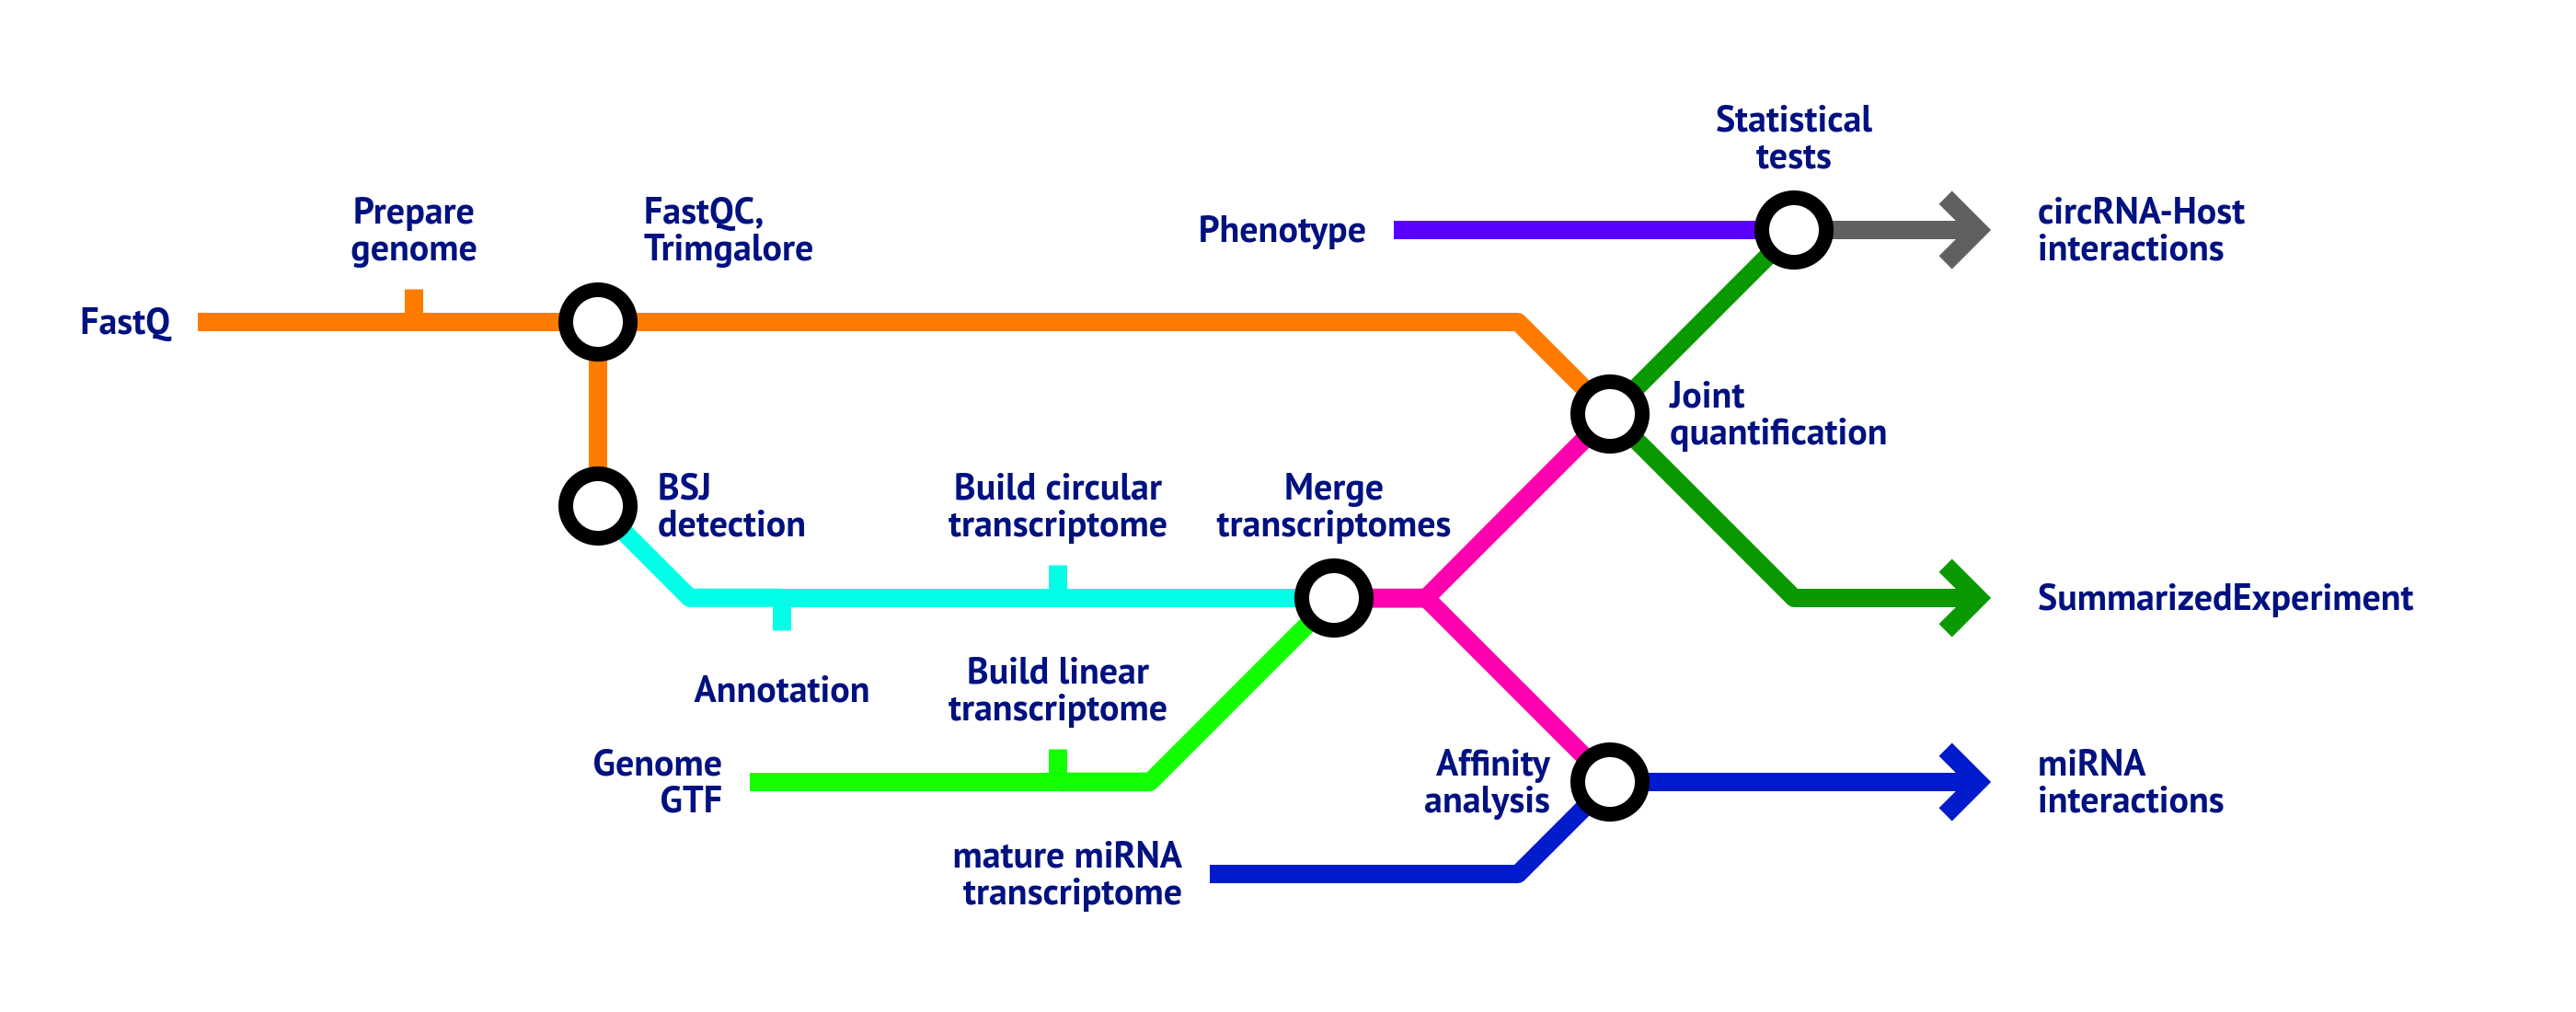
\includegraphics[width=\textwidth]{chapters/3_materials_and_methods/figures/nf-core_circrna.png}
    \caption{nf-core/circrna} % TODO: Add detailed caption
    \label{fig:circrna_pipeline}
\end{figure}

\subsection{\gls{crna} detection}
\label{subsec:circrna_detection}
From a molecular perspective, \gls{crna}s are similar to their linear
counterparts, with the primary distinction being their circular structure.
As explained in \cref{sec:circrna_biogenesis}, \gls{crna}s are derived from a
linear precursor (identical to linear RNA) that undergoes back-splicing to form
a loop.
Thus, the only way to computationally identify \gls{crna}s is by detecting
reads spanning the \gls{bsj}, which cannot be accounted for by canonical
forward splicing.
nf-core/circrna provides a total of seven tools for \gls{bsj}
detection.
However, only five of them are compatible with single-end sequencing data.
I will briefly discuss these five tools below.

\subsubsection{find\_circ (2013)}
Find\_circ is one of the pioneering tools for \gls{crna} detection,
specifically designed for identifying circular RNAs by leveraging RNA-seq data.
It employs a novel alignment strategy, splitting reads that do not map linearly
to the genome into smaller fragments, which are then re-aligned to detect
\gls{bsj}s\supercite{memczak_circular_2013}.
This tool does not rely on any known annotations and processes RNA-seq reads
using Bowtie, an efficient aligner for identifying \gls{bsj} reads.
One of its key features is that it filters for \gls{bsj} reads, removing those
that align entirely to the genome, which makes it stand out from methods
relying heavily on gene annotations\supercite{memczak_circular_2013}.

While it has been effective in many studies, it may not capture \gls{crna}s
with non-canonical splice signals, which can limit its detection
capabilities\supercite{sekar_circular_2018,liu_prkra_2022}.
Nonetheless, find\_circ remains a popular choice for researchers due to its
ease of use and integration with RNA-seq workflows.

\subsubsection{Segemehl (2014)}
Segemehl integrates a sensitive and flexible read-matching algorithm based on
enhanced suffix arrays (ESAs).
It identifies \gls{bsj} reads through split-read mapping, where the RNA-seq
data is aligned using a dynamic programming strategy that identifies splicing,
trans-splicing, and fusion transcripts.
Its major advantage over other tools is its ability to map reads containing
multiple split sites, which boosts sensitivity for detecting \gls{crna}s even
in complex cases like long reads or sequences with
errors\supercite{hoffmann_multi-split_2014}.

While Segemehl has shown promise in identifying \gls{crna}s, its performance
can vary depending on the specific dataset and experimental
conditions\supercite{gao_ciri_2015,zeng_comprehensive_2017}.

\subsubsection{DCC (2016)}
DCC relies on STAR as its underlying aligner, which maps RNA-seq reads to the
genome.
It uses a combination of filters to detect \gls{bsj}s by distinguishing
back-splice reads from linear splicing.
DCC integrates across replicates to minimize false positives and improve the
precision of \gls{crna} detection.
What sets DCC apart is its post-mapping step, where it not only detects
\gls{crna}s but also estimates their expression relative to the host gene using
read counts from junction and non-junction reads.
This makes it highly useful for comparing \gls{crna} expression across
conditions\supercite{cheng_specific_2016}.
DCC has been validated in numerous studies, demonstrating high reliability and
accuracy in \gls{crna} detection\supercite{paraboschi_interpreting_2018}.

\subsubsection{CIRCexplorer2 (2016)}
CIRCexplorer2 is another widely used tool that focuses on the detection of
\gls{crna}s by analyzing RNA-seq data.
It employs a unique strategy that combines both \gls{bsj} reads and linear RNA
reads to improve \gls{crna} identification.
CIRCexplorer2 has demonstrated robust performance in various studies, often
ranking high in comparative evaluations against other \gls{crna} detection
tools\supercite{zeng_comprehensive_2017,nicolet_circular_2018}.
Its ability to provide detailed annotations and quantifications of \gls{crna}s
makes it a valuable resource for researchers\supercite{hansen_comparison_2016}.
%TODO: Update

\subsubsection{CIRI2 (2018)}
CIRI2 improves upon the original CIRI\supercite{gao_ciri_2015} by using a
maximum likelihood estimation (MLE) based on multiple seed matching to detect
\gls{bsj} reads.
This algorithm is optimized for high sensitivity while maintaining a low false
discovery rate by filtering out false positives from repetitive sequences and
mapping errors.
It employs BWA-MEM for initial alignment, with CIRI2 distinguishing itself by
its efficient use of computational resources and ability to handle mixed read
lengths, making it faster and more memory-efficient compared to other
methods\supercite{gao_circular_2018}.

\subsection{\Glsfmtshort{crna} annotation}
In its minimal form, a \gls{crna} is defined by the chromosome it is located on
and the start and end position of the \gls{bsj}.
While this information is sufficient to uniquely identify a \gls{bsj}, it does
not provide any information about the gene or genes it is part of.
Furthermore, it does not give any information about the type of \gls{crna} it
is (types of \gls{crna} are described in \cref{sec:circrna_types}) and if it is
already has an entry in any \gls{crna} database.
While some tools like \gls{cex2} and \gls{dcc} provide their own annotation,
other tools like \gls{findcirc} and \gls{segemehl} do not.
To provide a consistent annotation for all \glspl{bsj}, \gls{nf-circrna} uses a
custom annotation process that will be described in the following sections.

\subsubsection{\gls{gtf}-based annotation}
\label{sec:gtf_annotation}
\gls{gtf} files are a common way to store genomic annotations like gene
locations and
transcript structures.
Such files are available for many reference genomes and can be used to identify
the genes and linear transcripts a \gls{crna} overlaps with.
This information can be used to infer the host gene(s) and the type of
\gls{crna}.

\begin{figure}[ht]
      \centering

      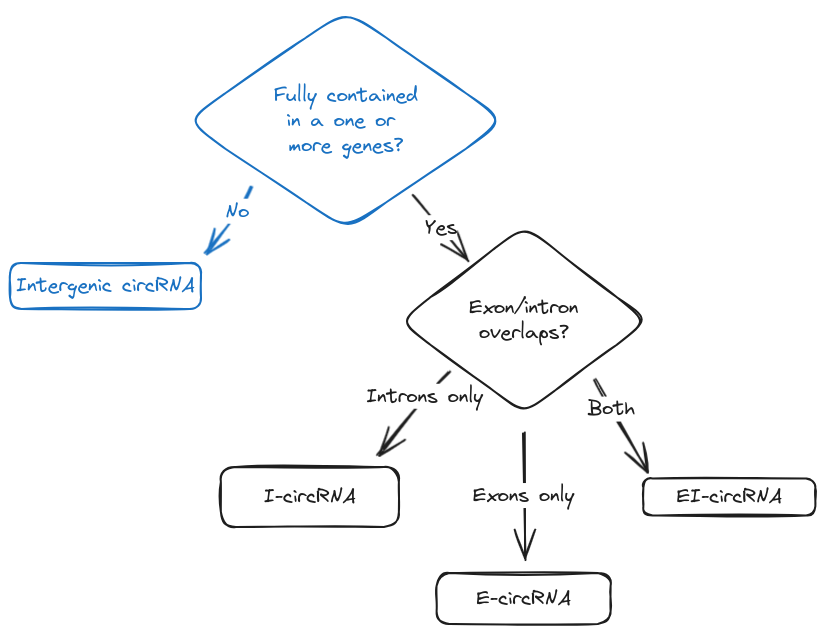
\includegraphics[width=\textwidth]{chapters/3_materials_and_methods/figures/annotation.png}
      \caption{Decision tree of the \gls{gtf}-based \gls{crna} type annotation}
      \label{fig:gtf_annotation}
\end{figure}

The \gls{nf-circrna} pipeline identifies the type of \gls{crna} as shown in
\cref{fig:gtf_annotation}: \begin{enumerate} \item If the \gls{crna} does not
            overlap with any gene, it is labeled as \gls{ig-crna}.
      \item If the \gls{crna} is fully contained in any gene, the following
            classification is performed:
            \begin{itemize}
                  \item If the \gls{crna} is fully contained in an exon, it is
                        labeled as \gls{e-crna}.
                  \item If the \gls{crna} is fully contained in an intron, it
                        is
                        labeled as \gls{i-crna}.
                  \item If the \gls{crna} spans both exonic and intronic
                        regions,
                        it is labeled as \gls{ei-crna}.
            \end{itemize}
\end{enumerate}

\subsubsection{Database-based annotation}
\label{sec:database_annotation}
In addition to \gls{gtf}-based annotation, \gls{nf-circrna} also provides
database-based annotation.
Databases like \gls{circbase} and \gls{circatlas} store information about known
\glspl{crna}, often including functional
information\supercite{glazar_circbase_2014,wu_circatlas_2023}.
Most \gls{crna} databases provide their stored \glspl{crna} in form of a
\gls{bed} file, providing a fairly unified interface for tools to process their
stored information in an automated fashion.
\gls{nf-circrna} allows the user to provide an arbitrary number of such
\gls{bed}
files for database-based annotation.
The pipeline identifies a match between a detected \gls{crna} and a database
entry, if the bi-directional overlap is at least 90\%.
This means that at least 90\% of the detected \gls{crna} must overlap with the
database entry and vice versa.

In this study, the following databases were used for annotation:

\paragraph{\Glsfmtlong{circbase}} \gls{circbase}, established in 2014, was one of the first
databases dedicated to \glspl{crna}.
It compiled data from nine large-scale studies, encompassing 92,375
\glspl{crna} from humans and key model
organisms\supercite{glazar_circbase_2014}.
Although \gls{circbase} was accessible at the beginning of this study, it has since
been taken offline.

\paragraph{\Glsfmtlong{circatlas}}
The latest version of \gls{circatlas} was released in early 2024 and offers a
more extensive dataset with three million vertebrate \glspl{crna}.
It covers ten species and 33 different tissues, providing valuable
cross-species conservation scores for researchers\supercite{wu_circatlas_2023}.

\subsection{\gls{crna} quantification}
\label{sec:crna_quantification}

While all \gls{bsj} detection tools quantify the number of reads
supporting each \gls{bsj}, there are several tools that focus on the
quantification of \glspl{crna} based on previously detected \glspl{bsj}.
nf-core/circrna offers two such tools: CIRIquant and
psirc-quant.

\subsubsection{CIRIquant}
\label{sec:ciriquant}
CIRIquant extends the CIRI (\Gls{crna} Identifier) framework, focusing on
accurate \gls{crna} quantification by re-aligning \gls{bsj} reads to a
pseudo-reference sequence.
Although it natively utilizes CIRI2 for \gls{bsj} detection, it can also
process \glspl{bsj} identified by other tools\supercite{zhang_accurate_2020}.
For each \gls{bsj}, CIRIquant constructs a pseudo \gls{crna} reference by
concatenating two copies of the sequence between the \gls{bsj} start and end
positions.
By comparing alignments to both the reference genome and the pseudo-reference
sequence, CIRIquant calculates the fraction of reads utilizing the \gls{bsj}
among those that span at least one of its
boundaries\supercite{zhang_accurate_2020}.
The output provided by CIRIquant is essentially the CPM (counts per million) of
reads supporting each \gls{bsj}, normalized by the total number of mapped reads
in the sample.

\subsubsection{psirc}
\label{sec:psirc}
As illustrated in \cref{fig:psirc_workflow}, psirc operates in two main phases:
first, the identification of \gls{bsj} and inference of full-length isoforms
(FLI); and second, the quantification of expression levels for the detected
isoforms\supercite{yu_quantifying_2021}.

\begin{figure}[ht] \centering

    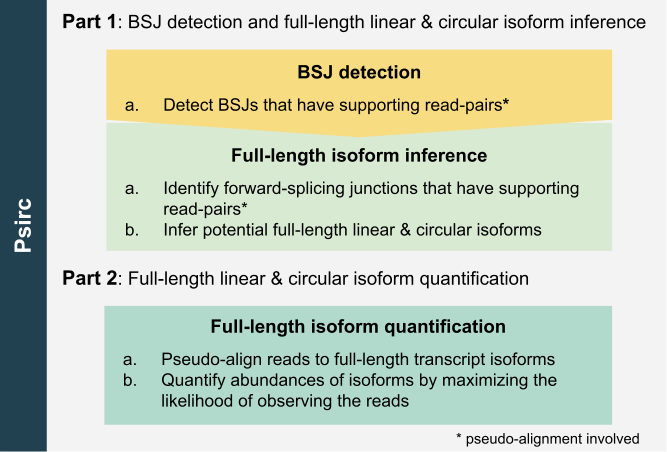
\includegraphics[width=0.5\textwidth]{chapters/3_materials_and_methods/figures/psirc_pipeline.png}
    \caption{psirc-workflow} \label{fig:psirc_workflow} \end{figure}

The initial phase of the workflow functions similarly to the implementation
described in \cref{sec:ciriquant}, with the added step of full-length isoform
inference.
However, this step requires paired-end sequencing data, which is not available
in this thesis.
While psirc's \gls{bsj} detection can be substituted with other tools, the FLI
inference step is more challenging to replace.
Previous studies have attempted to address this by using information from the
linear transcriptome to retain only exonic regions within the \gls{bsj} limits
\supercite{hoffmann_circrna-sponging_2023}.
If no exonic regions are present, the entire sequence is retained.
In contrast, the nf-core/circrna pipeline takes a different approach, retaining
the entire sequence within the \gls{bsj} boundaries, regardless of exonic
region presence.
This method avoids assumptions about the internal structure of the \gls{crna}.

For the quantification phase, psirc requires a combined transcriptome FASTA
file containing both linear and circular transcripts.
Psirc constructs a Transcript de Bruijn Graph (T-DBG) from this combined
transcriptome and utilizes Kallisto to jointly quantify the expression levels
of both transcript types\supercite{yu_quantifying_2021}.
This approach enables a direct comparison between linear and circular isoforms,
potentially offering deeper insights into the regulatory roles of \glspl{crna}
in gene expression.
Notably, psirc does not explicitly differentiate between reads spanning the
\gls{bsj} and those fully contained within it; instead, it relies on Kallisto's
likelihood maximization to distinguish between linear and circular
isoforms\supercite{yu_quantifying_2021}.

\subsection{\gls{mirna} interaction analysis}
The analysis of circular RNA (\gls{crna}) interactions with microRNAs (\gls{mirna}s)
is crucial for understanding the regulatory roles of \gls{crna}s in various
biological processes.
Two prominent tools used for predicting \gls{crna}-\gls{mirna} interactions are
MiRanda and TargetScan.
These tools leverage sequence complementarity and binding energy calculations
to identify potential \gls{mirna} binding sites within \gls{crna} sequences, thereby
elucidating their roles as competitive endogenous RNAs (ceRNAs).

\subsubsection{MiRanda}
MiRanda is a widely utilized algorithm that predicts \gls{mirna} targets based on
sequence complementarity and the stability of the RNA duplex formed between the
\gls{mirna} and its target.
It has been effectively employed in various studies to analyze \gls{crna}-\gls{mirna}
interactions.
For instance, Vromman et al.
noted that
MiRanda is often used alongside TargetScan to predict \gls{mirna} binding sites in
\gls{crna} sequences, contributing to a better understanding of \gls{crna}
functions
in gene regulation\supercite{vromman_closing_2021}.
Similarly, Zhang et al.
utilized
MiRanda in conjunction with TargetScan to predict microRNA response elements
(MREs) in differentially expressed \gls{crna}s, demonstrating its utility in
identifying significant interactions\supercite{zhang_microarray_2017}.

\subsubsection{TargetScan}
TargetScan, on the other hand, focuses on the identification of conserved \gls{mirna}
binding sites across species, which enhances the reliability of the predicted
interactions.
This tool has been integrated into various studies to explore the regulatory
networks involving \gls{crna}s and \gls{mirna}s.
For example, Jin et al.
employed MiRanda and TargetScan to predict interactions between \gls{crna}s and
\gls{mirna}s, reinforcing the hypothesis that \gls{crna}s can act as \gls{mirna}
sponges\supercite{jin_changes_2018}.
Furthermore, the combination of these tools allows researchers to construct
comprehensive \gls{crna}-\gls{mirna}-\gls{mrna} networks, elucidating the complex
regulatory mechanisms at play in various
diseases\supercite{he_construction_2021,zhang_construction_2021}.

\subsection{Downstream analyses}
\subsubsection{R-shiny}
\subsubsection{Dimensionality reduction}
\subsubsection{Pathway analysis}
\subsubsection{Differential expression analysis}
\subsubsection{Genome browser}

